%%% LaTeX Template: Two column article
%%%
%%% Source: http://www.howtotex.com/
%%% Feel free to distribute this template, but please keep to referal to http://www.howtotex.com/ here.
%%% Date: February 2011

%%% Preamble
\documentclass[	DIV=calc,%
							paper=a4,%
							fontsize=12pt,%
							onecolumn]{scrartcl}	 					% KOMA-article class

\usepackage{lipsum}													% Package to create dummy text
\usepackage[brazil]{babel}										% English language/hyphenation
\usepackage[protrusion=true,expansion=true]{microtype}				% Better typography
\usepackage{amsmath,amsfonts,amsthm}					% Math packages
\usepackage[pdftex]{graphicx}									% Enable pdflatex
\usepackage[svgnames]{xcolor}									% Enabling colors by their 'svgnames'
\usepackage[hang, small,labelfont=bf,up,textfont=it,up]{caption}	% Custom captions under/above floats
\usepackage{epstopdf}												% Converts .eps to .pdf
\usepackage{subfig}													% Subfigures
\usepackage{booktabs}												% Nicer tables
\usepackage{fix-cm}													% Custom fontsizes
\usepackage[utf8]{inputenc}
\usepackage[top=2.5cm, bottom=2.5cm, left=2.5cm, right=2.5cm]{geometry}
\usepackage[ddmmyyyy]{datetime}
\usepackage{pdfpages}
\addto\captionsenglish{%
	\renewcommand\tablename{Tabela}
	\renewcommand\figurename{Figura}
} 
 

 
%%% Custom sectioning (sectsty package)
\usepackage{sectsty}													% Custom sectioning (see below)
\allsectionsfont{%															% Change font of al section commands
	\usefont{OT1}{phv}{b}{n}%										% bch-b-n: CharterBT-Bold font
	}

\sectionfont{%																% Change font of \section command
	\usefont{OT1}{phv}{b}{n}%										% bch-b-n: CharterBT-Bold font
	}



%%% Headers and footers
\usepackage{fancyhdr}												% Needed to define custom headers/footers
	\pagestyle{fancy}														% Enabling the custom headers/footers
\usepackage{lastpage}	

% Header (empty)
\lhead{}
\chead{}
\rhead{}
% Footer (you may change this to your own needs)

%% ====================================
%% ====================================
%% mude o rodape  do projeto
%% ====================================
%% ====================================

\lfoot{\footnotesize \texttt{Projeto de Cabeamento estruturado para uma} \textbullet ~~Clínica}


\cfoot{}
\rfoot{\footnotesize página \thepage\ de \pageref{LastPage}}	% "Page 1 of 2"
\renewcommand{\headrulewidth}{0.0pt}
\renewcommand{\footrulewidth}{0.4pt}



%%% Creating an initial of the very first character of the content
\usepackage{lettrine}
\newcommand{\initial}[1]{%
     \lettrine[lines=3,lhang=0.3,nindent=0em]{
     				\color{DarkGoldenrod}
     				{\textsf{#1}}}{}}



%%% Title, author and date metadata
\usepackage{titling}															% For custom titles

\newcommand{\HorRule}{\color{DarkGoldenrod}%			% Creating a horizontal rule
									  	\rule{\linewidth}{1pt}%
										}

\pretitle{\vspace{-30pt} \begin{flushleft} \HorRule 
				\fontsize{50}{50} \usefont{OT1}{phv}{b}{n} \color{DarkRed} \selectfont 
				}

%% ====================================
%% ====================================
%% mude o titulo  do projeto
%% ====================================
%% ====================================

\title{Projeto de Cabeamento estruturado para uma Clínica}					% Title of your article goes here

%% ====================================



\posttitle{\par\end{flushleft}\vskip 0.5em}

\preauthor{\begin{flushleft}
					\large \lineskip 0.5em \usefont{OT1}{phv}{b}{sl} \color{DarkRed}}
\author{Lucas F. Concato, Odaír S. F. da Costa,Cassio Scheffer}  	% Author name goes here


\postauthor{\footnotesize \usefont{OT1}{phv}{m}{sl} \color{Black} 
					\\Universidade Tecnológica Federal do Paraná - Câmpus Cornélio Procópio 								% Institution of author
					\par\end{flushleft}\HorRule}

\date{}																				% No date




%%% Begin document
\begin{document}
\maketitle
\thispagestyle{fancy} 	
\thispagestyle{empty}		% Enabling the custom headers/footers for the first page 
% The first character should be within \initial{}




%% ====================================
%% ====================================
%% mude o resumo  do projeto
%% ====================================
%% ====================================

\initial{E}\textbfste modelo contém as informações necessárias para a criação um projeto de cabeamento estruturado para uma clínica. Utilizaremos a topologia do tipo estrela, pois atenderá as necessidades do nosso cliente, o qual trabalhará com sete salas disponíveis para atendimento e uma sala para armazenamento dos equipamentos, sendo todos alojados em apenas um andar, assim ficará melhor distribuído e organizado.}


%% ====================================
\begin{figure}
	\centering
	
\includegraphics{utfpr}
\end{figure}

\vspace{2cm}
\centerline{\textit{\textbf{\today}}}

\clearpage
    \renewcommand*\listfigurename{Lista de figuras}
\listoffigures





\clearpage
\renewcommand{\contentsname}{Sumário}
\tableofcontents
\clearpage

%% ====================================
%% ====================================
%% Inicio do texto
%% ====================================
%% ====================================
\section{Introdução}
Essa proposta tem por objetivo realizar a implementação de uma rede lógica para uma clínica, onde contará com sete salas disponíveis para a utilização dos colaboradores, todas equipadas com um notebook e uma impressora de rede, a cada duas salas haverá um roteador, afim de disponibilizar um sinal de WIFI para seus clientes e melhor atendê-los, constando assim 6 roteadores. Esse projeto inicial é foi montado para uma clínica a qual possui 14 colaboradores.

Escopo do projeto tem por intuito disponibilizar os seguintes itens:
\begin{itemize}
\item Rede Lógica – Infraestrutura de Rede Lógica;
\item Cabo Cm Cat6 – Vermelho Ral3020;
\item Calha de tomadas 8 tomadas 10A;
\item Organizador Horizontal (guia U);
\item Patch Cord Cat.6 1m vermelho – vermelho;
\item Path Panel 24P Cat. 6 UTP;
\item Switch Edge Core Ecs 4120 – 52t 10/100/1000 + 2 portas SFP 10GB Gerenciavel L2	
\item Switch Edge Core Ecs 4620 – 28F 10/100/1000 + 2 portas 1GB Gerenciavel L2
\end{itemize}
\subsection{Benefícios}
\begin{itemize}
 \item Uma melhora no compartilhamento e disponibilidade das informações entre os colaboradores e seus clientes.
\item Disponibilização de um ambiente onde seus clientes possam navegar com tranquilidade.
\item Melhor estruturação da empresa para eventuais mudanças.
\end{itemize}

\section{Requisitos}
\begin{itemize}

	\item 1 caixa de Cabo Cm Cat6 – Vermelho Ral3020 ("R$ 500,00$);
	\item 28 Calha de tomadas 8 tomadas 10A;
	\item 2 Organizador Horizontal (guia U);
	\item 30 Patch Cord Cat.6 1m vermelho – vermelho;
	\item 2 Path Panel 24P Cat. 6 UTP;
	\item 1 Switch Edge Core Ecs 4120 – 52t 10/100/1000 + 2 portas SFP 10GB Gerenciavel L2	
	\item 1 Switch Edge Core Ecs 4620 – 28F 10/100/1000 + 2 portas 1GB Gerenciavel L2
	
\end{itemize}	


\section{Usuários e Aplicativos}
O projeto foi feito especificamente para essa quantidade de funcionários devido a estrutura física do local não suportar mais, entretanto caso haja um crescimento, a empresa tem a intenção de realizar um novo projeto.
 

\subsection{Usuários}
\begin{itemize}
	\item 14 usuários fixos(colaboradores)
	\item clientes que estiverem presentes
\end{itemize}

\subsection{Aplicativos}
\begin{itemize}
	\item Sistema de gerenciamento da clínica, o qual contém todas as informações dos pacientes, agendamentos, histórico dos atendimentos, possui um nível elevado de prioridade e que em nenhum momento pode ficar offline, podendo causar grandes prejuízos financeiros.
	\item Arquivos compartilhados no servidor, a todo momento é realizado requisições ao servidor pelos funcionários para acessar e editar arquivos dos seus clientes.
\end{itemize}


\section{Estrutura predial existente}

Composto por 7 salas, sendo 6 de atendimento e 1 para recepção, e um outro lugar separado onde ficará instalado todos os equipamentos necessários. Estima-se aproximadamente 2 cabos de 10 metros saindo para as primeiras salas e aumentando em 10 metros para as demais salas.

\section{Planta Lógica - Elementos estruturados}

\subsection{Estado atual}

\begin{figure}
	\centering
	\makebox[\textwidth][c]{
		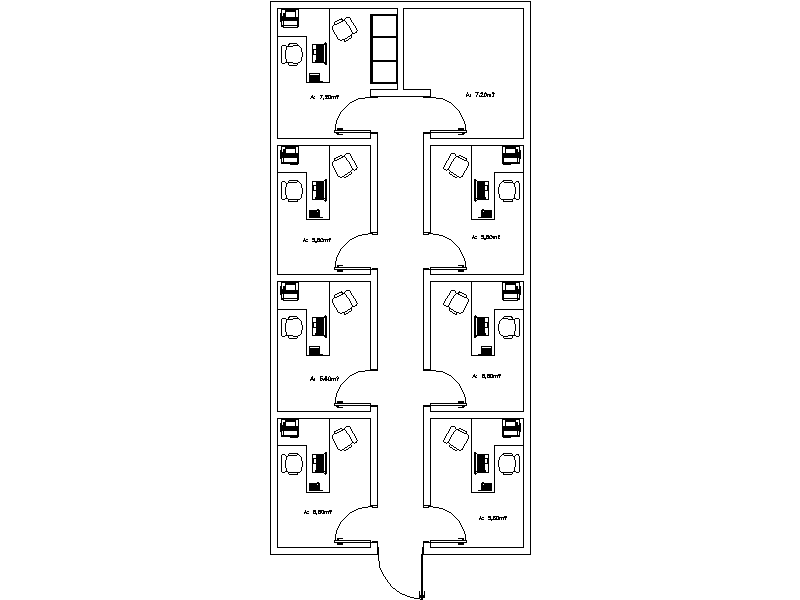
\includegraphics[height=\textheight]{planta}}
	\caption{Planta da clínica}
	\label{planta}
\end{figure}


\subsection{Memorial descritivo}

\begin{itemize}
	\item Execução e conclusão do projeto previsto para 45 dias após confirmação via contrato.
	\item 1 caixa de Cabo Cm Cat6 – Vermelho Ral3020;
	\item 28 Calha de tomadas 8 tomadas 10A;
	\item 2 Organizador Horizontal (guia U);
	\item 30 Patch Cord Cat.6 1m vermelho – vermelho;
	\item 2 Path Panel 24P Cat. 6 UTP;
	\item 1 Switch Edge Core Ecs 4120 – 52t 10/100/1000 + 2 portas SFP 10GB Gerenciavel L2	
	\item 1 Switch Edge Core Ecs 4620 – 28F 10/100/1000 + 2 portas 1GB Gerenciavel L2
	
\end{itemize}

\subsection{Identificação dos cabos}
Todos os cabos possuíram etiquetas informando com um código, "c"+número para computadores ou laptop's e "i"+número para impressoras.
\section{Implantação}
Quando o estabelecimento estiver preparado para as instalações, dará início pela montagem dos racks, em seguida, instalação dos condutores e cabos necessários, e somente após a conclusão, iniciará a etapa de certificação, e no final haverá uma revisão de todo o projeto, afim de certificar de possíveis falhas e identificar melhorias. 

\section{Plano de certificação}
Toda a rede será certificada logo após a sua implementação.

\section{Plano de manutenção}
Programada revisão dos equipamentos e instalações a cada 6 meses.

\subsection{Plano de expansão}
Não é viável ao momento. 

\section{Risco}
Não identificado.

\section{Orçamento}
\begin{itemize}

	\item 1 caixa de Cabo Cm Cat6 – Vermelho Ral3020 (RS 580,00);
	\item 28 Calha de tomadas 8 tomadas 10A (RS 1960,00);
	\item 2 Organizador Horizontal (guia U) (RS 200,00);
	\item 30 Patch Cord Cat.6 1m vermelho – vermelho (RS 3000,00);
	\item 2 Path Panel 24P Cat. 6 UTP (RS 1700,00);
	\item 1 Switch Edge Core Ecs 4120 – 52t 10/100/1000 + 2 portas SFP 10GB Gerenciavel L2 (RS 8500,00);
	\item 1 Switch Edge Core Ecs 4620 – 28F 10/100/1000 + 2 portas 1GB Gerenciavel L2 (RS 8580,00);
	
\end{itemize}	


\section{Recomendações}
Orientado ao cliente que caso tenha a intenção de expandir, será necessário um novo ambiente devido as limitações físicas do atual estabelecimento.


\end{document}
